% GENERATED by figures/make_cg_tee_artifacts.py from evidence/cg_tee_*.json.
% Every number is recomputed at build time; edit the script, not this file.
\section{The Per-Seed Record Behind Table~\ref{tab:results}}\label{sec:perseed}
Table~\ref{tab:results} prints three aggregates. The archive also holds the 15 per-seed records they were computed from, in \texttt{evidence/cg\_tee\_checkpoint.json} (byte-identically mirrored as \texttt{experiments/results/cg\_tee\_checkpoint.json}; 5 distinct contents across the shipped \texttt{cg\_tee*.json} paths), plus a separate real-API family. Recomputing means from the per-seed values reproduces the printed aggregates to $1.1e-16$, so the arithmetic of the summary is sound. What does not survive the per-seed view is the caption's reading of it, and two of the surrounding sentences.

\begin{table}[ht]\centering\small
\caption{Mean $\gamma_{T\to V}$ per arm, recomputed from the 15 per-seed records and set beside the value the aggregate file records, its bootstrap CI, and the recomputed change relative to the standard arm. Rows are written by \texttt{figures/make\_cg\_tee\_artifacts.py}; the $\Delta$ column is not a tolerance, it is the floating-point difference between two computations of the same mean.}
\label{tab:perarm}
\begin{tabular}{lrrrrc}\toprule
Arm & $n$ & recomputed & recorded & rel.\ to standard & recorded 95\% CI \\ \midrule
Standard TTRL & 15 & 0.143 & 0.143 & +0.0\% & [0.127, 0.159] \\
CG alone & 15 & 0.719 & 0.719 & +402.7\% & [0.663, 0.772] \\
CG + TEE & 15 & 0.574 & 0.574 & +301.4\% & [0.511, 0.627] \\
\bottomrule\end{tabular}\end{table}

\begin{figure}[ht]\centering
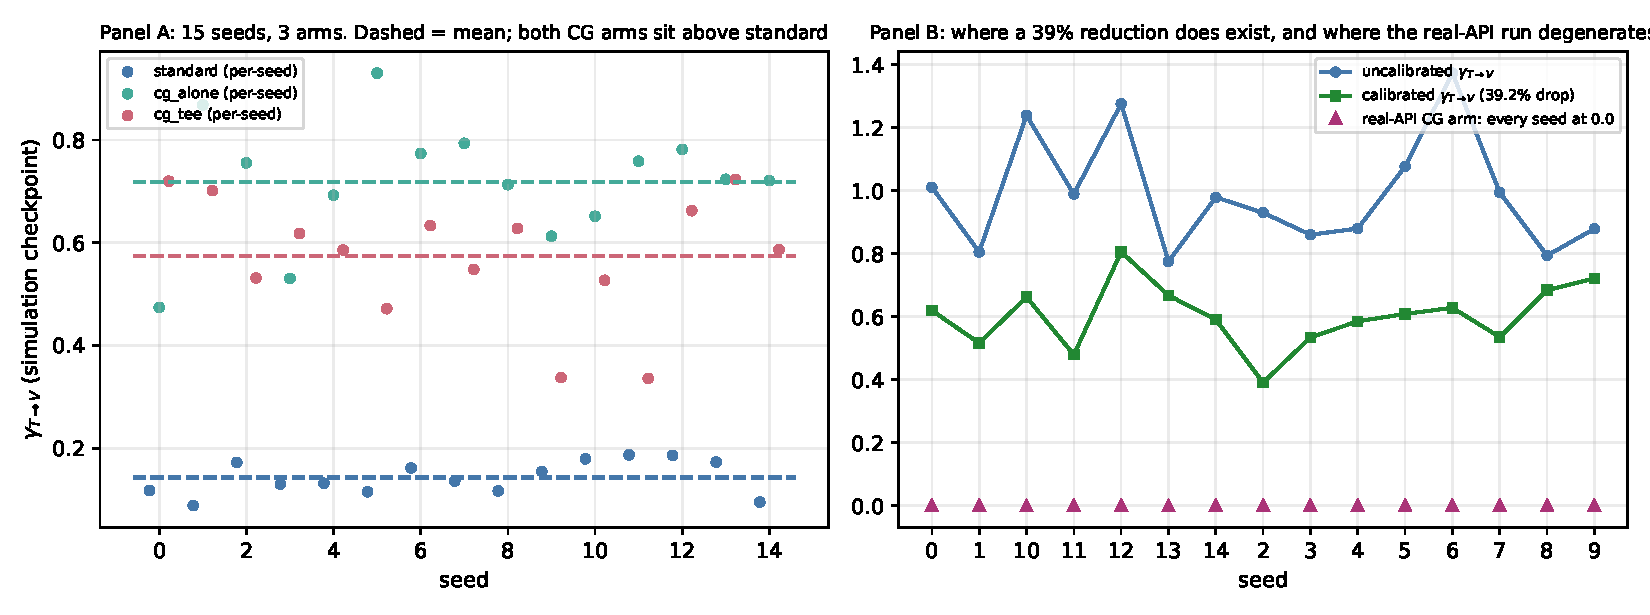
\includegraphics[width=0.94\linewidth]{fig_cg_tee_seeds.pdf}
\caption{Panel A: all 15 per-seed $\gamma_{T\to V}$ values for the three simulation arms, with arm means dashed. Both confidence-gated arms lie above the standard arm on every simulation seed. Panel B: two numerically lower outputs that are not valid mitigation evidence --- the uncalibrated versus calibrated blocks of \texttt{cg\_tee\_final\_results.json}, whose provenance is unresolved, and the real-API CG arms, which are parser-degenerate with $\gamma=0$ and $H=1$ on all 15 seeds. Generated from \texttt{evidence/cg\_tee\_checkpoint.json}, \texttt{cg\_tee\_final\_results.json} and \texttt{cg\_tee\_real\_results.json}.}
\label{fig:perseed}
\end{figure}

\noindent\textbf{The direction is the opposite of the caption's.} Standard $\gamma_{T\to V}$ averages 0.143, CG alone 0.719 (a 403\% increase, seed by seed) and CG+TEE 0.574 (301\%). The aggregate file encodes the same fact as \texttt{delta\_gamma\_pct} of -433.4 under a \emph{reduction} sign convention, so a negative percentage is an increase in coupling. Read either way, the gated arms do not reduce coupling in this artifact.

\noindent\textbf{Where the 39\% scalar comes from.} The 39.2\% value is the $\gamma_{T\to V}$ difference between the uncalibrated and calibrated blocks of \texttt{cg\_tee\_final\_results.json}. It is not a CG+TEE estimate. Even for the calibration contrast, the artifact's provenance and model identity are unresolved, so the number is a recorded scalar rather than a validated intervention effect.

\noindent\textbf{The CV column has no per-seed carrier.} The recorded \texttt{cv} values are 0.192, 0.134, 0.174. Four definitions were tried against them (sample and population coefficient of variation, and the standard deviation, of \texttt{gamma} and of \texttt{H}), with nearest gaps 0.030, 0.016, 0.029. None reproduces the recorded number, and the direction in which a smaller \texttt{cv} is an improvement is not stated anywhere in the artifact. A claim that TEE ``improves CV'' is therefore not checkable from this archive, and is not repeated here.

\noindent\textbf{Which run each condition belongs to.} 1 of the 15 JSON records in the archive names an executor and an evaluator: \texttt{experiments/results/cg\_tee\_local\_smoke.json} at \texttt{qwen2.5:3b-instruct-q4\_K\_M}/\texttt{qwen2.5:3b-instruct-q4\_K\_M}. That is the 3-seed local smoke run. The $N{=}15$ simulation and real-API files carry a config of \texttt{n\_seeds}, \texttt{n\_rounds}, \texttt{k\_tee}, \texttt{alpha} and \texttt{tau} only, so the model pair stated in Experimental Design is recorded in prose files and in the manuscript, not in the per-seed data. This is the kind of gap a reviewer cannot close from the artifact, and it is why the per-seed table below reports seeds rather than claiming a model-level comparison.

\begin{table}[ht]\centering\small
\caption{Every per-seed $\gamma_{T\to V}$ in \texttt{cg\_tee\_checkpoint.json}, as read. This is the whole simulation dataset: 15 seeds, 3 arms, 45 numbers.}
\label{tab:seeddata}
\begin{tabular}{rrrr}\toprule
Seed & Standard & CG alone & CG + TEE \\ \midrule
0 & 0.1177 & 0.4742 & 0.7199 \\
1 & 0.0882 & 0.8683 & 0.7015 \\
2 & 0.1722 & 0.7554 & 0.5313 \\
3 & 0.1303 & 0.5306 & 0.6178 \\
4 & 0.1317 & 0.6928 & 0.5858 \\
5 & 0.1153 & 0.9303 & 0.4717 \\
6 & 0.1614 & 0.7738 & 0.6335 \\
7 & 0.1361 & 0.7937 & 0.5482 \\
8 & 0.1169 & 0.7131 & 0.6281 \\
9 & 0.1547 & 0.6127 & 0.3375 \\
10 & 0.1791 & 0.6516 & 0.5269 \\
11 & 0.1870 & 0.7588 & 0.3358 \\
12 & 0.1861 & 0.7817 & 0.6625 \\
13 & 0.1729 & 0.7236 & 0.7232 \\
14 & 0.0952 & 0.7209 & 0.5867 \\
\bottomrule\end{tabular}\end{table}

